% ============================================================================
\section{Materials and Methods}
\label{sec:methods}
% ============================================================================

Every calculation in this thesis runs on a laptop. The quantum processor is
simulated on purpose, so that every intermediate quantity, including the full
noisy density matrix, can be inspected. The design rule is that each stage of
the pipeline has an answer known by independent means attached to it, and the
number reported for each check is a residual rather than a pass or fail flag.
Figure~\ref{fig:pipeline} shows the chain from the Hamiltonian to a measured
number, with the check attached at each link, and Table~\ref{tab:checks}
collects the residuals. This section describes each link in turn.

% ---------------------------------------------------------------- pipeline
\begin{figure}[t]
  \centering
  \begin{tikzpicture}[
      font=\small,
      nohyph/.style={execute at begin node={\hyphenpenalty=10000\exhyphenpenalty=10000}},
      box/.style={nohyph, draw=black!70, rounded corners=2pt, fill=blue!4, align=center,
                  text width=5.6cm, minimum height=0.85cm, inner sep=3pt},
      chk/.style={nohyph, draw=black!45, rounded corners=2pt, fill=black!3, align=left,
                  text width=6.2cm, minimum height=0.85cm, inner sep=3pt, font=\footnotesize},
      result/.style={nohyph, draw=black!70, rounded corners=2pt, fill=orange!8, align=center,
                  text width=5.3cm, minimum height=0.85cm, inner sep=3pt},
      flow/.style={-{Stealth[length=2mm]}, thick, black!70},
      link/.style={densely dotted, black!50},
      node distance=0.32cm]
    \node[box] (a) {Continuum Schwinger model, Eq.~\eqref{eq:lagrangian}};
    \node[box, below=of a] (b) {Staggered fermions on $N=4$ sites, open boundaries};
    \node[box, below=of b] (c) {Gauss's law solved; gauge field eliminated};
    \node[box, below=of c] (d) {Jordan--Wigner: 14 Pauli strings on 4 qubits};
    \node[box, below=of d] (e) {Second-order Trotter circuit, compiled to
                                $\{$RZ, SX, X, CX$\}$, 32 CX per step};
    \node[box, below=of e] (f) {Gate error (exact density matrix), then readout error};
    \node[box, below=of f] (g) {One $\Zop{}$-basis distribution gives
                                $\nu$, $\langle\Lop{n}\rangle$, $\hat Q$ and CP};
    \node[result, below=0.55cm of g, xshift=-1.75cm] (h) {Error budget and crossover;
                                failure threshold and its prediction from
                                $\mathrm{Var}(Q)$};
    \node[result, right=0.4cm of h] (i) {SKQD ground state: sampled bitstrings,
                                classical diagonalisation};
    \foreach \u/\v in {a/b, b/c, c/d, d/e, e/f, f/g} \draw[flow] (\u) -- (\v);
    \draw[flow] (g.south -| h.north) -- (h.north);
    \draw[flow] (g.south -| i.north) -- (i.north);

    \node[chk, right=0.55cm of b] (cb) {Strong-coupling limit $E_0=-mN/2$: 0\\
                                       Free fermions, all 16 levels: \num{9e-16}};
    \node[chk, right=0.55cm of c] (cc) {Gauss's law an identity: 0;\quad $[\Hop,\hat Q]$: 0};
    \node[chk, right=0.55cm of d] (cd) {Three constructions: 0\\
                                       Hellmann--Feynman: \num{4e-12}};
    \node[chk, right=0.55cm of e] (ce) {Exponents 1.036, 2.003 (predicted 1, 2)\\
                                       CP preserved without noise: \num{5e-16}};
    \node[chk, right=0.55cm of f] (cf) {Noise-free limit: \num{1.5e-14}; closed forms
                                       for readout and global channel};
    \node[chk, right=0.55cm of g] (cg) {Quoted standard errors match the scatter of
                                       repeated runs to 3\,\%};
    \foreach \u in {b, c, d, e, f, g} \draw[link] (\u) -- (c\u);
  \end{tikzpicture}
  \caption{The computational pipeline (left) and the independent check attached
  to each stage (right; residuals from Table~\ref{tab:checks}). The two outputs
  at the bottom are the dynamics error budget, with the crossover, the failure
  threshold and its prediction from charge conservation
  (Section~\ref{sec:budget-method}), and the ground state prepared by
  sample-based Krylov diagonalisation (Section~\ref{sec:skqd}), which reuses the
  same Trotter circuits.}
  \label{fig:pipeline}
\end{figure}

\subsection{Software}

The code is a Python 3.11 package, \texttt{schwinger}, with exact linear algebra
in NumPy~2.4 and SciPy~1.17~\cite{harris2020,virtanen2020}, circuits in
Qiskit~2.5~\cite{javadi2024}, noisy simulation in Qiskit Aer~0.17, and figures
in Matplotlib~3.11~\cite{hunter2007}; the exact versions are pinned in a lock
file. Each figure in this thesis is produced by one script that also prints the
residuals it relies on, every entry of Table~\ref{tab:checks} is printed by
\texttt{scripts/09\_verification\_table.py}, and all random sampling uses fixed
seeds, so rerunning a script reproduces its output. A suite of 476 tests
compares every module against independently known answers. The code, tests and
scripts are kept in a Git repository, private at the time of writing and
available from the author on request.

Two conventions cause silent errors if confused, and both are fixed in one
place in the code. A Pauli string such as \texttt{ZIZI} is read left to right as
site~1 to site~$N$, with site~1 the most significant tensor factor. Qiskit uses
the same label order but numbers its qubits in reverse, so lattice site $n$ is
Qiskit qubit $N-n$. Every gate index passes through a single conversion
function, and a test confirms that Qiskit's own operator, built from the labels
of Table~\ref{tab:pauli}, equals the NumPy matrix entry by entry.

\subsection{Exact reference and verification}
\label{sec:verification}

At $N = 4$ the Hamiltonian is a $16\times 16$ Hermitian matrix, diagonalised
exactly. Exact time evolution uses its spectral decomposition,
$|\psi(t)\rangle = \sum_k e^{-iE_k t}|k\rangle\langle k|\psi(0)\rangle$, so one
diagonalisation serves every time. These exact results are the reference for
every approximate result in the thesis, so the Hamiltonian itself is checked
first, in ways that fail for different reasons.

The matrix is built three ways that share nothing beyond the Pauli matrices
and the staggering sign $(-1)^n$: from the expanded Pauli list
of Table~\ref{tab:pauli}; directly, by squaring each $\Lop{n}$ as a matrix
without any algebra; and from the fermionic form Eq.~\eqref{eq:H_fermion}, with
fermion operators built through the Jordan--Wigner transformation. The three
agree to \num{9e-16} or better at every parameter set tried, and exactly at the
thesis parameters. This catches errors in the hand expansion of $\Lop{n}^2$ and
in the Jordan--Wigner signs, but not an error shared by all three, such as a
wrong starting Hamiltonian. Analytic limits test the physics instead. With no
hopping ($w = 0$) the Hamiltonian is diagonal and the bare vacuum minimises both
remaining terms, so $E_0 = -mN/2$ exactly; this tests the mass and electric
terms and is blind to the hopping. With no mass or field ($m = J = 0$) only the
hopping survives, a tight-binding chain with single-particle energies
$2w\cos[k\pi/(N+1)]$, $k = 1,\dots,N$, whose subset sums must reproduce all
sixteen levels; this tests the hopping and the Jordan--Wigner string and is
blind to the electric term.

A further check ties the observable to the Hamiltonian. The condensate computed
from the ground-state vector and the condensate computed as $N^{-1}dE_0/dm$ from
a finite difference of eigenvalues agree to \num{4e-12}, the size of the
finite-difference error. The Hellmann--Feynman theorem guarantees this
agreement for any Hamiltonian of the form $\Hop_0 + m\hat V$, so it shows only
that the observable and the mass term match in sign, staggering and
normalisation; the hopping and electric terms are covered by the constructions
and limits above. Before any of this, the Jordan--Wigner machinery was learned
on the transverse-field Ising model, whose full spectrum is known in closed
form~\cite{sachdev2011}; all $2^N$ levels were reproduced to \num{3e-14} for
$N = 2$, 4, 6 and 8. Finally, the Gauss's-law identity, $[\Hop,\hat Q] = 0$ and the
two CP maps of Section~\ref{sec:symmetries} are verified as operator identities
on the full space.

\begin{table}[tbp]
  \centering
  \caption{Verification checks at $N = 4$, $m = 0.5\,w$, $J = w$ unless stated,
  all printed by \texttt{scripts/09\_verification\_table.py}. Unless marked,
  each entry is the largest absolute disagreement between a computed quantity
  and an independently known answer, with energies in units of $w$; $0$ means
  exact agreement in floating point. Fitted exponents are given with their
  predicted values. Statistical checks are ratios of measured to predicted
  spread, which should be 1, or deviations in standard errors.}
  \label{tab:checks}
  \small
  \begin{tabular}{p{10.6cm}l}
    \toprule
    Check & Residual \\
    \midrule
    \multicolumn{2}{l}{\emph{Hamiltonian}} \\
    Pauli expansion vs.\ direct matrix construction & $0$ \\
    Fermionic form through Jordan--Wigner vs.\ spin form & $0$ \\
    Strong coupling, $E_0 = -mN/2$ at $w = 0$ & $0$ \\
    Free fermions, all 16 levels at $m = J = 0$ & \num{9e-16} \\
    Hellmann--Feynman: condensate vs.\ $N^{-1}dE_0/dm$ & \num{4e-12} \\
    Gauss's law as an operator identity; $[\Hop,\hat Q]$ & $0$; $0$ \\
    $[\mathrm{CP},\Hop]$ inside $Q = 0$ (largest element on the full space: 5) & $0$ \\
    CP maps $\hat\rho_n \to -\hat\rho_{N+1-n}$ and $\Lop{n} \to \Lop{N-n} - \hat Q$ & $0$; $0$ \\
    Drift of $\langle\Hop\rangle$ in exact evolution, $t \le 12$, $m/w = 0$ to 2 & \num{5e-15} \\
    Transverse-field Ising warm-up, full $2^N$ spectrum, $N = 2$, 4, 6, 8 & \num{3e-14} \\
    \midrule
    \multicolumn{2}{l}{\emph{Circuits}} \\
    Qiskit operator from Pauli labels vs.\ NumPy matrix & $0$ \\
    Circuit state vs.\ $e^{-i\Hop t}|\mathrm{vac}\rangle$ at $t = 2$, 4000 second-order steps & \num{7e-8} \\
    State-error exponent at $t = 3$, first / second order (predicted 1 / 2) & 1.036 / 2.003 \\
    Exponent of the bias on $\nu$ at $t = 1.76$, second order (predicted 2) & 2.002 \\
    Noiseless-circuit CP asymmetry, $\delta t = 0.5$, $0.25$, $0.1$, three times & \num{5e-16} \\
    \midrule
    \multicolumn{2}{l}{\emph{Noise}} \\
    Density-matrix simulation vs.\ statevector, no noise & \num{1.5e-14} \\
    Logical-frame route vs.\ Aer route, no noise & \num{2.9e-15} \\
    Infidelity convention vs.\ Qiskit's average gate fidelity (relative) & \num{4e-12} \\
    Readout: closed form $\tfrac12 + (1-2q)(\nu - \tfrac12)$, $q = 0.01$ to 0.2 & \num{6e-17} \\
    Readout: classical model vs.\ Aer, $q = 0.08$, $2\times10^5$ shots, worst bin & $1.9\,\sigma$ \\
    Global channel, $p = 0.005$ to 0.1 per step for 18 steps: $F_Q$ vs.\ $(1-p)^{18}$ & \num{7e-16} \\
    Logical-frame dephasing, $p = 0.01$, 0.05: $\mathrm{Var}(Q)$; $A_{\mathrm{CP}}$ (must vanish) & \num{9e-34}; \num{7e-16} \\
    Fully depolarising CX: $|\mathrm{Var}(Q) - N/4|$ & $0$ \\
    \midrule
    \multicolumn{2}{l}{\emph{Statistics, budget and ground state}} \\
    Scatter of 400 simulated runs / quoted standard error, $\nu$ and $\mathrm{Var}(Q)$ & 0.97 to 1.01 \\
    Mean squared error of 600 runs / $(b^2 + \sigma^2)$ & 0.999 \\
    Threshold prediction on data that obey the global model & \num{2e-16} \\
    Dip under four channels, $\delta t = 0.1$ to 0.3: largest $D - D_{\mathrm{noiseless}}$ (must be $< 0$) & \num{-2e-4} \\
    SKQD on the full neutral sector vs.\ exact ground energy & \num{4e-16} \\
    SKQD bound: smallest $E(S) - E_0$, 62 proper subspaces (must be $> 0$) & \num{3.2e-3} \\
    SKQD bias at 15 shots per step: exact / 20\,000 Monte Carlo runs
      & \num{1.020e-3} / \num{1.002(40)e-3} \\
    \bottomrule
  \end{tabular}
\end{table}

\subsection{Trotterised time evolution}

The Hamiltonian is split into three groups whose members commute among
themselves,
\begin{equation}
  \Hop = \Hop_Z + \Hop_{\mathrm{e}} + \Hop_{\mathrm{o}},
\end{equation}
where $\Hop_Z$ contains every $\Zop{}$ and $\Zop{}\Zop{}$ term (the mass and
electric energy, all diagonal), $\Hop_{\mathrm{e}}$ the hopping on the two outer
bonds, (1,2) and (3,4), and $\Hop_{\mathrm{o}}$ the hopping on the middle bond,
(2,3). The labels are the usual even and odd split with bonds counted from zero,
as in the code. Adjacent bonds share a site and do not commute, which is why the
hopping is split this way. Each group exponentiates exactly, so the only error
comes from the splitting. The first-order step is
$U_1(\delta t) = e^{-i\Hop_Z\delta t}e^{-i\Hop_{\mathrm{e}}\delta t}e^{-i\Hop_{\mathrm{o}}\delta t}$,
and the second-order, symmetric step used throughout is
\begin{equation}
  \label{eq:strang}
  U_2(\delta t) = e^{-i\Hop_Z\delta t/2}\,e^{-i\Hop_{\mathrm{e}}\delta t/2}\,
                  e^{-i\Hop_{\mathrm{o}}\delta t}\,
                  e^{-i\Hop_{\mathrm{e}}\delta t/2}\,e^{-i\Hop_Z\delta t/2}.
\end{equation}
A circuit to time $t$ applies the step $n$ times, with $n$ an integer, so a
nominal step $\delta t$ means $n = \mathrm{round}(t/\delta t)$ steps of $t/n$.
The error at fixed $t$ then scales as $\delta t$ for the first-order formula and
as $\delta t^2$ for the second~\cite{suzuki1976,childs2021}. The scaling is a
sharper test than the size of the error, because an implementation can be
accurate at one step size and still scale wrongly. The state error is defined
as the largest amplitude difference from $e^{-i\Hop t}|\mathrm{vac}\rangle$
after the global phase is removed. Fitting its logarithm against $\log\delta t$
at $t = 3$, for $\delta t$ from 0.3 to 0.0094, gives exponents of 1.036 and
2.003; the bias in the particle density at $t = 1.76$, for $\delta t$ from 0.088
to 0.011, gives 2.002.

Each exponential becomes gates directly. With the standard rotations
$\mathrm{R}_P(\theta) = e^{-i\theta P/2}$ for a Pauli operator $P$, a term
$c\,\Zop{n}$ is an $\mathrm{RZ}(2c\,\delta t)$ rotation and a term
$c\,\Zop{n}\Zop{n'}$ an $\mathrm{RZZ}(2c\,\delta t)$. On one bond,
$\tfrac12 w(\Xop{}\Xop{} + \Yop{}\Yop{})$ becomes $\mathrm{RXX}(w\,\delta t)$
followed by $\mathrm{RYY}(w\,\delta t)$; the two commute on the same bond, so
the pair is exact. For noise simulation the circuit is compiled to the native
gate set of superconducting devices, $\{\mathrm{RZ}, \mathrm{SX}, \mathrm{X},
\mathrm{CX}\}$, where SX is the square root of X and CX is the controlled-NOT
gate. In this set every RZZ, RXX and RYY costs two CX gates, and one
second-order step contains 32 CX, 24 SX and 53 RZ gates
(Figure~\ref{fig:trotterstep}). Compilation uses Qiskit's transpiler at
optimisation level 1 with a fixed seed and no coupling map, so any two qubits
are assumed to be directly coupled, as on a trapped-ion processor. On a chip
with nearest-neighbour coupling the RZZ between sites 1 and 3 would need extra
SWAP gates, and the CX counts here would rise. The RZ gates are implemented in
software on superconducting hardware, as a change of the phase reference of
later pulses, and carry no error~\cite{mckay2017}. The circuit whose gates are
counted and the circuit whose gates carry noise are the same compiled object.

\begin{figure}[t]
  \centering
  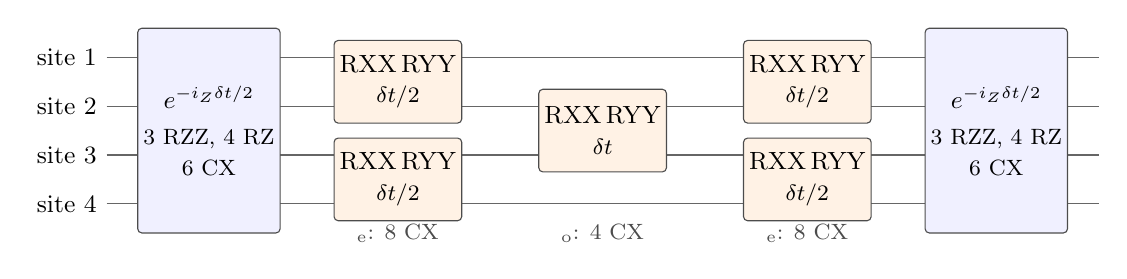
\begin{tikzpicture}[font=\small, x=1cm, y=0.62cm,
      gate/.style={draw=black!70, fill=white, rounded corners=1.5pt, align=center,
                   minimum width=1.55cm, inner sep=2pt},
      diag/.style={gate, fill=blue!6},
      hop/.style={gate, fill=orange!10}]
    \foreach \q in {1,...,4} {
      \draw[black!60] (0,-\q) -- (12.6,-\q);
      \node[left] at (0,-\q) {site \q};
    }
    \node[diag, minimum height=2.6cm] at (1.3,-2.5)
      {$e^{-i\Hop_Z\delta t/2}$\\[2pt]\footnotesize 3 RZZ, 4 RZ\\\footnotesize 6 CX};
    \node[hop, minimum height=1.05cm] at (3.7,-1.5) {RXX\,RYY\\\footnotesize $\delta t/2$};
    \node[hop, minimum height=1.05cm] at (3.7,-3.5) {RXX\,RYY\\\footnotesize $\delta t/2$};
    \node[hop, minimum height=1.05cm] at (6.3,-2.5) {RXX\,RYY\\\footnotesize $\delta t$};
    \node[hop, minimum height=1.05cm] at (8.9,-1.5) {RXX\,RYY\\\footnotesize $\delta t/2$};
    \node[hop, minimum height=1.05cm] at (8.9,-3.5) {RXX\,RYY\\\footnotesize $\delta t/2$};
    \node[diag, minimum height=2.6cm] at (11.3,-2.5)
      {$e^{-i\Hop_Z\delta t/2}$\\[2pt]\footnotesize 3 RZZ, 4 RZ\\\footnotesize 6 CX};
    \node[font=\footnotesize, black!70] at (3.7,-4.6) {$\Hop_{\mathrm{e}}$: 8 CX};
    \node[font=\footnotesize, black!70] at (6.3,-4.6) {$\Hop_{\mathrm{o}}$: 4 CX};
    \node[font=\footnotesize, black!70] at (8.9,-4.6) {$\Hop_{\mathrm{e}}$: 8 CX};
  \end{tikzpicture}
  \caption{One second-order Trotter step, Eq.~\eqref{eq:strang}, on four
  qubits. Diagonal layers (blue) apply the mass and electric terms. Hopping
  layers (orange) apply $\tfrac12 w(\Xop{}\Xop{}+\Yop{}\Yop{})$ to the outer bonds
  for half a step, the middle bond for a full step, and the outer bonds again.
  Compiled to $\{\mathrm{RZ},\mathrm{SX},\mathrm{X},\mathrm{CX}\}$ the step costs
  32 CX gates, the number that sets how fast gate error accumulates.}
  \label{fig:trotterstep}
\end{figure}

\subsection{Measurement and shot noise}

Every observable in Section~\ref{sec:theory}, together with $\hat Q$, is
diagonal in the computational basis, so each is a function $x_b$ of the measured
bitstring $b$ alone. One circuit measured once in the $\Zop{}$ basis therefore
gives the physics and the diagnostics together, with no extra circuits. An
$M$-shot estimate of $\langle x\rangle$ is the sample mean, and its standard
error is
\begin{equation}
  \label{eq:sigma}
  \sigma_x = \sqrt{\frac{1}{M}\sum_b p_b\,\bigl(x_b - \langle x\rangle\bigr)^2},
  \qquad \langle x\rangle = \sum_b p_b x_b ,
\end{equation}
where $p_b$ is the probability of outcome $b$~\cite{taylor1997}. The particle
number of a single shot takes the values 0, 1, 2, 3 or 4, not just 0 and 1, so
the binomial formula $\sqrt{p(1-p)/M}$ does not apply and Eq.~\eqref{eq:sigma}
is the general form. For $\mathrm{Var}(Q)$ the standard error of a sample
variance is used, $\sqrt{(\mu_4 - \mu_2^2)/M}$, with $\mu_2 = \mathrm{Var}(Q)$
and $\mu_4$ the second and fourth central moments of $Q$ per shot.

The distribution $p_b$ is known exactly in simulation, so Eq.~\eqref{eq:sigma} is
evaluated exactly rather than estimated from one noisy sample, and shot noise
enters the budget as a computed number rather than as a fluctuation that has to
be averaged away. When a realistic data set is needed, $M$ outcomes are drawn
from $p_b$ by multinomial sampling, which is statistically identical to running
the circuit $M$ times. Over 400 independent simulated data sets of 256 and of
2048 shots, the actual scatter of the estimates is between 0.97 and 1.01 times
the quoted standard error, for both $\nu$ and $\mathrm{Var}(Q)$.

\subsection{Hardware noise models}

Gate errors are modelled as depolarising channels attached to the physical
gates of the compiled circuit. Acting on the $d$-dimensional space of a gate's
own qubits,
\begin{equation}
  \mathcal{E}(\rho) = (1-\lambda)\,\rho + \lambda\,\frac{I_d}{d}\otimes\mathrm{Tr}_g\,\rho,
\end{equation}
where $\mathrm{Tr}_g$ traces out those qubits, $d = 4$ for a CX gate and $d = 2$
for SX and X. The strength is quoted as the average gate infidelity $\epsilon$,
the number obtained from randomised benchmarking and reported on hardware data
sheets~\cite{magesan2011}, which is related to $\lambda$ by
$\epsilon = \lambda(d-1)/d$~\cite{nielsen2010,magesan2011}. Confusing the two
would misstate every threshold by a factor $4/3$, so the conversion is checked
against Qiskit's own average-gate-fidelity routine. The two-qubit error
$\epsilon_2$ is swept from $10^{-5}$ to $3\times 10^{-2}$, a range that brackets
the two-qubit error of $4\times10^{-3}$ reported for the trapped-ion processor
used by Rosanowski \emph{et al.}~\cite{rosanowski2025}. The single-qubit error
is set to $\epsilon_1 = \epsilon_2/10$. This ratio is an assumption. With it,
the 24 SX gates of each step add less than a tenth of the error that its 32 CX
gates do, and its effect on the failure threshold defined below is tested by
repeating the threshold sweep with $\epsilon_1 = 0$ and
$\epsilon_1 = 0.3\,\epsilon_2$.

As a control, the CX depolarising channel is replaced in some runs by
independent phase flips, $\rho \to (1-\epsilon_2)\rho + \epsilon_2\Zop{}\rho\Zop{}$
on each of its two qubits, with flips of probability $\epsilon_1$ after SX and
X. Here $\epsilon_2$ is a flip probability, not an average infidelity, so the
two models are compared through the fidelity they produce, Eq.~\eqref{eq:FQ}
below, and not at equal $\epsilon_2$.

Readout error is modelled as an independent bit flip with probability $q$ on
each qubit, applied as a $2\times 2$ confusion matrix to each qubit's axis of the
outcome distribution. It acts only on the classical record, after the state has
been measured, so it is applied afterwards to the computed noisy distribution and its
bias stays separate from the gate error. A symmetric flip maps every
$\langle\Zop{n}\rangle$ to $(1-2q)\langle\Zop{n}\rangle$, so the particle density
becomes $\tfrac12 + (1-2q)(\nu - \tfrac12)$; the code reproduces this closed form
to \num{6e-17}, and over $2\times 10^5$ sampled shots it agrees with Aer's own
readout-error model to within $1.9$ standard deviations in every outcome bin.
Readout error can be corrected by inverting the confusion
matrix~\cite{bravyi2021}, so it is reported as its own term in the budget rather
than folded into the gate error.

The noisy state is computed exactly. Aer's density-matrix simulator carries the
full $16\times 16$ density matrix through every noisy gate and returns the exact
outcome probabilities, with no sampling. The gate-error bias of any observable is
then an exact number, and shot noise is added afterwards through
Eq.~\eqref{eq:sigma}.

A second route applies noise once per Trotter step to the state of the four
lattice sites, called here the logical frame to distinguish it from errors
inside a compiled gate. The step unitary is taken as a $16\times16$ matrix and
the noise is applied with NumPy matrix products, bypassing Aer and the
transpiler. This logical-frame route implements the phenomenological model
Martinez \emph{et al.}\ fitted to their data, a phase flip with probability $p$
on each qubit per step~\cite{martinez2016}, and a global depolarising channel
$\rho \to (1-p)\rho + pI/16$ per step. At zero noise it agrees with the Aer
route to \num{2.9e-15}. It exists as a control for the diagnostics, for the
reason given in Section~\ref{sec:diagnostics}. Four kinds of noise strength
appear and are kept apart: the average infidelity $\epsilon$ of a gate
($\lambda$ is its channel parameter), the readout flip probability $q$, the
probability $p$ per Trotter step of the logical-frame channels, and the
fidelity $F$ of a whole circuit.

Not modelled are amplitude damping, coherent errors such as a systematically
over-rotated gate, and errors correlated between qubits or between steps.
Amplitude damping drives every qubit toward $|0\rangle$, an occupied site here,
and its end point $|0000\rangle$ is a pure state with $Q = 2$ and
$\mathrm{Var}(Q) = 0$, so the global-model reading of $\mathrm{Var}(Q)$ in the
next subsection would fail for it.

\subsection{Symmetry diagnostics}
\label{sec:diagnostics}

From the same $\Zop{}$-basis data, three diagnostics are computed: the charge
variance $\mathrm{Var}(Q) = \langle\hat Q^2\rangle - \langle\hat Q\rangle^2$,
the leakage $1 - P(Q = 0)$ out of the six-state neutral sector, which is the
quantity Martinez \emph{et al.}\ reported~\cite{martinez2016}, and the CP
asymmetry $A_{\mathrm{CP}} = \langle\Lop{1}\rangle - \langle\Lop{3}\rangle$.
Without hardware noise all three vanish exactly, at any step size, because
every factor of the Trotter step conserves $\hat Q$ and commutes with CP in the
neutral sector (Section~\ref{sec:symmetries}).

Turning a violation into a prediction needs a model of the noise. The simplest
is a global depolarising channel, $\rho \to F\rho + (1-F)I/16$, under which every
diagonal observable moves linearly toward its maximally mixed value with the
same weight $F$~\cite{vovrosh2021,urbanek2021}. The ideal state has
$\mathrm{Var}(Q) = 0$ and the maximally mixed state has $\mathrm{Var}(Q) = N/4$,
so the model gives
\begin{equation}
  \label{eq:FQ}
  F_Q = 1 - \frac{\mathrm{Var}(Q)}{N/4},
\end{equation}
and an analogous estimate from the leakage. Both are exact for a global channel.
Real gate noise is local, not global, so Eq.~\eqref{eq:FQ} is a model whose
accuracy is one of the things this thesis measures. Only the charge variance is
turned into a prediction. The CP asymmetry vanishes on the maximally mixed
state, where $\langle\Lop{1}\rangle = \langle\Lop{3}\rangle = -\tfrac12$, so a
global channel cannot move it and it has no analogue of Eq.~\eqref{eq:FQ};
under gate noise it first grows and then returns to zero. It is reported as a
check and is not used as a predictor.

The diagnostics have a blind spot, and the logical-frame route exposes it. A
$\Zop{}$ error on the logical state commutes with $\hat Q$, so dephasing between
Trotter steps leaves $\mathrm{Var}(Q)$ exactly zero while the particle density
drifts far from its noiseless value. Uniform dephasing also commutes with CP,
so the CP asymmetry stays zero as well. Dephasing on the CX gates of the compiled
circuit, by contrast, does break charge conservation: a compiled RXX or RYY is
wrapped in single-qubit basis changes, so its CX gates act in a rotated frame,
and a $\Zop{}$ error on either of them becomes an $\Xop{}$ or $\Yop{}$ error on
the logical state. Whether an error is visible to the diagnostic therefore
depends on where in the compiled circuit it occurs as well as on its type.

\subsection{The error budget}
\label{sec:budget-method}

For a diagonal observable at time $t$ and step size $\delta t$, four outcome
distributions are computed exactly, each differing from the last by one source of
error: $p^{\mathrm{exact}}$ from $e^{-i\Hop t}$, $p^{\mathrm{Trot}}$ from the
noiseless circuit, $p^{\mathrm{gate}}$ from the same circuit with gate noise, and
$p^{\mathrm{meas}}$ after readout error. The biases telescope,
\begin{equation}
  \label{eq:budget}
  \langle x\rangle^{\mathrm{meas}} - \langle x\rangle^{\mathrm{exact}}
  = b_{\mathrm{Trot}} + b_{\mathrm{gate}} + b_{\mathrm{read}},
\end{equation}
with $b_{\mathrm{Trot}} = \langle x\rangle^{\mathrm{Trot}} - \langle x\rangle^{\mathrm{exact}}$,
$b_{\mathrm{gate}} = \langle x\rangle^{\mathrm{gate}} - \langle x\rangle^{\mathrm{Trot}}$
and $b_{\mathrm{read}} = \langle x\rangle^{\mathrm{meas}} - \langle x\rangle^{\mathrm{gate}}$,
so the three biases add to the total exactly, by construction. The split itself
is a choice. Because the gate bias is defined on the Trotterised circuit, any
interplay between Trotter and gate error is counted as gate error, which matches
how an experiment is designed: the circuit is fixed first and then run on noisy
hardware. The shot noise $\sigma$ follows from $p^{\mathrm{meas}}$ through
Eq.~\eqref{eq:sigma}, and the root-mean-square error of a single $M$-shot
measurement is $\sqrt{b^2 + \sigma^2}$, with $b$ the total bias: the mean
squared error of an estimator is its squared bias plus its
variance~\cite{cai2023}. As a check that the estimator, the sampling code and
Eq.~\eqref{eq:sigma} agree with one another, 600 simulated 500-shot experiments
at $\epsilon_2 = 10^{-3}$ and $q = 0.02$ have a mean squared deviation from the
exact answer of 0.999 times $b^2 + \sigma^2$. Because the samples are drawn from
the same $p^{\mathrm{meas}}$, this confirms the bookkeeping, not the
completeness of the noise model.

Two times recur below. Starting from the bare vacuum, the exact particle density
rises to its first maximum, $\nu = 0.463$ at $t_{\mathrm{p}} = 0.89$, and falls to
its first minimum, $\nu = 0.133$ at $t_{\mathrm{t}} = 1.76$, as pairs recombine.

\emph{The crossover.} The crossover step $\delta t_\times$ is the step at which
the Trotter bias in $\nu(t)$, with no hardware error, falls to the shot-noise
uncertainty $\sigma(M)$ of Eq.~\eqref{eq:sigma}, computed from the full outcome
distribution rather than sampled. It is located by
linear interpolation in $\log\delta t$ between neighbouring grid points
$\delta t = t/n$, at $t = 3$ (every $n$ from 2 to 32, then coarser up to 256)
and at $t_{\mathrm{t}}$ (14 values of $n$ from 2 to 64), for $M = 256$, 1000 and
4096 shots.

\emph{The optimal step.} For a 1000-shot measurement of $\nu(t_{\mathrm{t}})$
with readout error $q = 0.01$, the error $\sqrt{b^2 + \sigma^2}$ is evaluated on
the same 14 step sizes at $\epsilon_2 = 0$, $3\times10^{-4}$, $10^{-3}$ and
$3\times10^{-3}$, and the optimum is the grid point with the smallest error. At
the optimum, the share of each source is its square divided by
$b_{\mathrm{Trot}}^2 + b_{\mathrm{gate}}^2 + b_{\mathrm{read}}^2 + \sigma^2$,
for $\nu$ and for the outer and middle link fields.

\emph{The failure threshold.} The signal is the recombination dip
\begin{equation}
  \label{eq:dip}
  D = \nu(t_{\mathrm{p}}) - \nu(t_{\mathrm{t}}),
  \qquad
  \sigma_D = \sqrt{\sigma_{\mathrm{p}}^2 + \sigma_{\mathrm{t}}^2}.
\end{equation}
Depolarising noise drives the state toward the maximally mixed state, where
$\nu = \tfrac12$ at every time and $D = 0$. In every noise sweep in this thesis,
for each of the four channels modelled and all three step sizes, $D$ shrinks
from its noiseless value as the noise grows, and can fall below zero, but never
exceeds that value (Table~\ref{tab:checks}); a dip that survives was therefore
not created by the noise. This is an observation about the channels modelled
rather than a theorem. Coherent errors, which are not modelled, could in
principle shift or mimic the dip. The failure threshold $\epsilon^\ast$ is the smallest two-qubit error at
which $D \le 2\sigma_D$, found by interpolation in $\log\epsilon_2$ on a
36-point grid from $10^{-5}$ to $3\times10^{-2}$, for nominal step sizes
$\delta t = 0.1$, $0.2$ and $0.3$ and for $M = 10^3$ and $10^4$ shots. The number
of steps is rounded separately at each time; for $\delta t = 0.2$ that is four
steps to $t_{\mathrm{p}}$ and nine to $t_{\mathrm{t}}$. The measurement times
are fixed at the extrema of the exact evolution, as an experiment would choose
them from theory. Readout error is left out of the threshold and of its
prediction. It would add about $Nq(1-q)$, roughly 0.04 at $q = 0.01$, to
$\mathrm{Var}(Q)$ and multiply $D$ by $1-2q$, so on hardware the confusion
matrix would have to be inverted before Eq.~\eqref{eq:FQ} is applied.

\emph{Predicting the threshold.} An experiment has data at one noise level
$\epsilon_0$ only, and the prediction uses those data alone, in four steps.
First, Eq.~\eqref{eq:FQ} turns the measured charge variance into a fidelity
$F_Q$ at each of the two measurement times. Second, the global model is
assumed, so the measured distribution $p$ is inverted to an estimate of the
ideal one, $p^{\mathrm{ideal}} = [p - (1-F_Q)/16]/F_Q$. Third, the fidelity is
assumed to decay exponentially with gate error, $F(\epsilon) =
e^{-\kappa\epsilon}$, with $\kappa = -\ln F_Q/\epsilon_0$ fixed separately at
each time. Fourth, $p^{\mathrm{ideal}}$ is degraded with $F(\epsilon)$ at every
other $\epsilon$ to predict $D$ and $\sigma_D$ there, and the crossing of the
predicted $D$ with $2\sigma_D$ is the predicted threshold. Nothing in this
procedure uses the exact answer, and on synthetic data that obey the global
model it reproduces the true dip to \num{2e-16}. In the main comparison
$\mathrm{Var}(Q)$ at $\epsilon_0$ is computed from the full, unsampled noisy
distribution, so the test isolates the error of the global model from the shot noise on the
diagnostic. A real experiment would have $M$-shot data at $\epsilon_0$, so the
prediction is repeated on 200 data sets of 1000 shots sampled from that
distribution, which gives the scatter a single run would show. Comparing the
prediction with the threshold found by sweeping $\epsilon_2$ directly, for
$\epsilon_0$ near $\epsilon^\ast/10$ and $\epsilon^\ast/3$, is the test of the
third question in Section~\ref{sec:contribution}. The same comparison is
repeated with dephasing on the CX gates, the second gate-noise model.

\subsection{Ground state by sample-based Krylov diagonalisation}
\label{sec:skqd}

The ground state is prepared with SKQD, following Yu
\emph{et al.}~\cite{yu2025} and its application to the Schwinger model by
Rosanowski \emph{et al.}~\cite{rosanowski2025}. The reference state is the bare
vacuum, the ground state of the mass and electric terms, which Rosanowski
\emph{et al.}\ use as the initial state for their runs up to 30 qubits. The
circuits prepare $U(\delta t)^k|\mathrm{vac}\rangle$ for $k = 1,\dots,K$, with
$U(\delta t)$ either one second-order Trotter step of the full Hamiltonian,
Eq.~\eqref{eq:strang}, which reuses the dynamics circuits directly, or a step of
the hopping terms alone, of the kind Rosanowski \emph{et al.}\ use. Each circuit
is measured $M$ times. Bitstrings with nonzero total charge are discarded, which
costs nothing because $\hat Q$ is diagonal, and the distinct neutral bitstrings
from all $K$ steps, together with the reference, form a set $S$. The
Hamiltonian restricted to the span of $S$ is diagonalised classically, and its
lowest eigenvalue and eigenvector give the energy and the chiral condensate.
Because this is an exact diagonalisation inside a subspace, the estimate
satisfies $E_{\mathrm{SKQD}} \ge E_0$ for every possible $S$, however noisy the
sampling~\cite{kanno2023}. The bound holds on all 63 nonempty subsets of the
neutral sector, with a smallest margin of \num{3.2e-3} among the 62 proper ones.

Noise therefore cannot push the energy below the truth, but a finite number of
shots can miss an important bitstring and push it above~\cite{miura2026}. At
$N = 4$ this bias can be computed exactly. Let $p_k(b)$ be the outcome
distribution of the $k$-th circuit. For the sampled set to lie inside a set $T$
of neutral bitstrings, every one of the $M$ shots at every step must avoid the
neutral bitstrings outside $T$, so
\begin{equation}
  \label{eq:skqd}
  P(S \subseteq T) = \prod_{k=1}^{K}\Bigl(1 - \sum_{b \notin T} p_k(b)\Bigr)^{M}
\end{equation}
for every $T$ that contains the reference, and zero otherwise. The sum runs
over neutral bitstrings only; shots on charged bitstrings are discarded and do
no harm. Inclusion and exclusion over the $2^6 = 64$ subsets of the neutral
sector convert Eq.~\eqref{eq:skqd} into the probability that the sampled set is
exactly $S$, and the expected SKQD energy is the probability-weighted average of
the subspace energies. This exact result agrees with 20\,000 simulated SKQD runs
(Table~\ref{tab:checks}) and replaces Monte Carlo averaging in everything that
follows.

The hopping-only step needs one caution. Rosanowski \emph{et al.}\ write it as
$\exp[i(dt/4)\sum_n(\Xop{n}\Xop{n+1} + \Yop{n}\Yop{n+1})]$, which turns each
bond half as far as $\mathrm{RXX}(w\,\delta t)\,\mathrm{RYY}(w\,\delta t)$ does
at the same number, and their four-qubit run started from $|0011\rangle$ at
different parameters~\cite{rosanowski2025}. The SKQD runs therefore use
both $w\,\delta t = 0.77$, the value they chose, and $w\,\delta t = 0.385$, the
rotation it gives in their convention, and the comparison is with the kind of
step they use rather than with their circuit.

\subsection{Simulation parameters}

The physical parameters are those of Section~\ref{sec:parameters} and the
initial state is the bare vacuum. Trotter steps are second order unless stated
otherwise. The scaling test uses $\delta t$ from 0.0094 to 0.3 at $t = 3$. The
crossover uses $\delta t$ from 0.012 to 1.5 at $t = 3$ and, together with the
full budget, from 0.028 to 0.88 at $t_{\mathrm{t}}$. The threshold uses nominal
steps $\delta t = 0.1$, 0.2 and 0.3. Shot counts run from 256 to $10^4$ for the
dynamics and from 2 to 500 per Krylov step for SKQD; two-qubit gate errors run
from $10^{-5}$ to $3\times10^{-2}$ with $\epsilon_1 = \epsilon_2/10$; the
readout error in the budget is $q = 0.01$. SKQD uses $K = 4$ full Trotter steps
of $\delta t = 0.3$, without gate error and with $\epsilon_2 = 3\times10^{-3}$,
and a single hopping-only step of $w\,\delta t = 0.77$ or 0.385.
